\def\mb#1{\mathbb{#1}}
\newcommand{\ol}[1]{\overline{#1}}
\newcommand{\tbf}[1]{\textbf{#1}}

\newcommand\ccup{\mathop{\cup}}
\renewcommand{\dist}{\operatorname{dist}}
\newcommand{\id}{\operatorname{Id}}

\def\bar{\begin{array}}
\def\ear{\end{array}}
\newcommand{\Vol}{\operatorname{Vol}}

\task{Геометрическая вероятность}

Пункты этой задачи связаны с расположениями различных случайно взятых геометрических фигур. Что в каждом конкретном случае следует подразумевать под случайной фигурой того или иного вида, находится во власти решающего задачу, хотя, безусловно, требует обоснований. Одно можно сказать наверняка: вероятность --- это число от 0 до 1.
\begin{enumerate}
\item Пусть на плоскости задана квадратная решётка со стороной 1. Возьмём число $\varepsilon>0$ и вокруг точек решётки построим круги радиуса $\varepsilon$. Какова вероятность для случайной точки не попасть в объединение этих кругов?

\item На плоскость, расчерченную параллельными прямыми на расстоянии $h$  друг от друга падает случайный отрезок длины меньшей или равной $a$. Какова вероятность того, что этот отрезок пересечёт какую-то прямую? А каково математическое ожидание числа точек пересечения?
\item Та же задача, но теперь вместо отрезка на плоскость попадает крестик --- пара отрезков одинаковой фиксированной длины $a$, пересекающихся в своих центрах и перпендикулярных друг-другу. А что будет, если угол между отрезками не равен $\text{π}/2$?
\item Пусть дан некий круг радиуса $r$. Какова вероятность того, что конец отрезка длины $a$ лежит за пределами круга, если это случайный отрезок, чья середина лежит в круге?
\item Пусть плоскость замощена одинаковыми параллелограммами. На плоскость кидают случайный параллелограмм, среди тех 
\begin{description}
\item[а)] у которых площадь меньше или равна $S$.
\item[б)] у которых длина сторон меньше $a$.
\item[в)] у которых длины диагоналей меньше $a$.
\end{description}
Какова вероятность того, что вершина какого-то параллелограмма из замощения лежит в случайном параллелограмме?
\item А если рассмотреть случайный эллипс с такими условиями?
\item Рассмотрим случайный четырёхугольник с длинами сторон $a, b, c, d$. Какова вероятность, что он будет содержать точку из решётки? Какова вероятность, что он будет пересекаться с набором параллельных линий, расстояние между которыми равно $h$?
\item А что такое случайный $n$-угольник на плоскости c какими-то ограничениями? Какова вероятность для него содержать некоторую точку из решётки или пересекаться с семейством параллельных прямых?
\end{enumerate}


\task{Гипернатуральные числа}
\begin{enumerate}
\item Рассмотрим натуральные числа $n\neq 1$, $m_1$ и $m_2$.  Покажите, что $n^{m_1}-1 \,\,\vdots \,\, n^{m_2}-1$ тогда и только тогда, когда $m_1\,\, \vdots\,\, m_2$.\
\item Покажите, что для всех взаимнопростых чисел $m$ и $n$ существуют такие натуральные $k$ и $l$, что 
$ m^l-1 \,\,\vdots \,\, n$ и $n^k-1 \,\,\vdots \,\, m$.
\item Гипернатуральным числом назовём отображение из множества простых чисел $\mb{P}$ в множество $\mb{N}\cup\{0,\infty\}$. Естественным образом каждому натуральному числу можно сопоставить такое отображение, а именно, если $n=p_1^{\alpha_1}\dots p_n^{\alpha_n}$, где $p_i$ - различные простые, то соответствующее отображение задано формулой
$$ n(q)=\begin{cases}
\alpha_i,& q=p_i\\
0,& \text{иначе}
\end{cases}
$$
Также можно определить произведение, наименьшее общее кратное и наибольший общий делитель по следующим формулам:
$$ x_1 \cdot x_2 (q)=x_1(q)+x_2(q) ,$$
$$ \lcm(x_1,x_2)(q)=\max{(x_1(q),x_2(q))} ,$$
$$ \gcd (x_1, x_2)(q)=\min(x_1(q), x_2(q)) .$$
Будем говорить, что $x \,\,\vdots \,\, y$, если $\forall q\in \mb{P}\,\, x(q)\geq y(q)$.
Рассмотрим некоторое множество $A$ гипернатуральных чисел. Определим наименьшее общее кратное всех элементов из $A$ по формуле $\lcm (A)(q)= \sup\limits_{x\in A} \{x(q)\}$.
Теперь для гипернатурального числа $x$ и натурального $n$ определим
$$n^x-1= \lcm\left(\{n^m-1\, |\, m\in\mb{N},\, x\,\,\vdots\,\,m\}\right).$$
Решите следующие задачи:
\begin{description}
\item[а)] Вычислите $3^x-1$, $5^x-1$ и, в целом, $p^x-1$, где $p$-простое, а $x=(\infty, \infty, \dots)$.
\item[б)] Верно ли, что $n^x-1=n^y-1$ тогда и только тогда, когда $x=y$, где $x$ и $y$ гипернатуральные, $n\in\mb{N}$ .
\item[в)] Покажите, что уравнение $3^x-1=5^y-1$ неразрешимо в гипернатуральных числах. Аналогично покажите, что уравнение $3^x-1=11^y-1$ не имеет гипернатуральных решений.
\end{description}
\item Пусть $l^{\infty}=\lcm(\{l^n\,|\, n\in\mb{N}\})$. Попробуйте найти $p^{l^{\infty}}\!\!-1$ для некоторых простых $p$ и $l$.
\item Попробуйте разобрать случай уравнения $p^x-1=l^y-1$ для бесконечных серий простых чисел или дайте ответ для произвольных простых.
\item Бывают ли решения у уравнения $n^x-1=m^y-1$, когда $n$ и $m$ взаимнопростые натуральные числа? А когда не взаимнопростые?
\item Попробуйте решить другие уравнения в гипернатуральных числах, например, $n^x-a=n^y-b$.
\end{enumerate}



\task{Шоколадки}

Мальчик Коля пришёл в магазин выбирать шоколадку в поход. Так как вкусам своих товарищей он не видел возможности угодить, то Коля решил из всех шоколадок выбрать ту, которую проще всего поделить поровну. А именно, пусть шоколадка представляет собой прямоугольник $a\times b$, $a, b \in \mb{N}$, состоящий из $a\cdot b$ долек. Колю интересуют те формы шоколадок, где число долек делится поровну между участниками похода. Но вот беда, Коля точно не знает, сколько людей идёт в поход.
\begin{enumerate}
\item Считая, что в походе с одинаковой вероятностью могут оказаться от $2$ до $10$ человек, найдите все такие формы шоколадок из не более чем 100 долек, количество долек в которых с наибольшей вероятностью будет делиться на количество участников похода. Сколько различных конфигураций подойдёт? А если не более 50-ти долек?
\item При заданных ограничениях на размер шоколадки и на количество участников похода, те шоколадки, которые с наибольшей вероятностью делятся поровну, будем называть оптимальными. Решение с наименьшим числом долек будем назвать минимальной оптимальной шоколадкой.
\begin{description}
\item[а)] Покажите, что при фиксированном максимальном числе участников похода и росте ограничения на число шоколадок размер минимальной оптимальной шоколадки стабилизируется. Как описать размер (количество долек) минимальной шоколадки в зависимости от ограничения на число человек? Оцените, с какого места ограничение на размер не имеет значения.
\item[б)] Покажите, что при фиксированной верхней оценке на размер шоколадки и росте возможного числа людей, количество долек в минимальной шоколадке стабилизируется. Опишите и оцените размер минимальной шоколадки после стабилизации.
\item[в)] Сколько различных конфигураций для минимальных шоколадок из пунктов а) и б)?
\end{description}

\item Опишите алгоритм построения оптимальной шоколадки при заданных ограничениях. Какова сложность Вашего алгоритма?
\item Допустим теперь, что в магазине бывают не все шоколадки, а только вида $a\times b$, где $b\geq a\geq \varepsilon b$, для некоторого фиксированного $\varepsilon\leq 1$. Изменится ли количество долек в минимальной оптимальной шоколадке с таким условием? Оцените количество оптимальных шоколадок, удовлетворяющих этому условию.
\item Рассмотрим ситуацию, когда каждый из $d$ людей, которым Коля предложил идти в поход, пойдут в него --- $i$-ый с вероятностью $p_i\leq 1$. Будучи несколько ленивым, Коля хочет найти не самое оптимальное, а $\varepsilon$-оптимальное решение, то есть такую шоколадку, которая делится нацело между участниками с вероятностью в $\varepsilon\leq 1$ раз меньше, чем для оптимальной шоколадки.
Предложите свои варианты решения этой задачи, если:
\begin{description}
\item [а)] Для всякого $1\leq i\leq d\,$ $p_i=p<1$.
\item [б)] $\varepsilon$ достаточно маленькое ($\varepsilon=\frac{1}{100}$).
\end{description}

\end{enumerate}



\task{Матрицы и периоды}
\begin{enumerate}
\item Рассмотрим целочисленную матрицу $2\times 2$ 
$$\left(\begin{matrix}
1 & 1 \\
0 & 1 
\end{matrix}\right).$$
Возьмём некоторый целочисленный вектор $\left(\begin{smallmatrix} x  \\ y \end{smallmatrix}\right)$, натуральное число $n$ и построим последовательность
$$x_k=\left(\begin{matrix}
1 & 1 \\
0 & 1 
\end{matrix}\right)^k \left(\begin{matrix} x \\ y \end{matrix}\right) \mod n.$$
Здесь и далее под записью $\mod n$ подразумевается взятие остатка от деления на $n$.
Покажите, что эта последовательность будет чисто периодической, то есть существует такое $m\in \mb{N}$ со свойством $x_{k+m}=x_k$ для любого $k\in\mb{N}$. Каков период этой последовательности в зависимости от $x$, $y$ и $n$?
\item Рассмотрим целочисленную матрицу, некоторый начальный вектор и натуральное число $n$. Рассмотрим последовательность, аналогичную предыдущему пункту

$$x_k=\left(\begin{matrix}
a & b \\
c & d
\end{matrix}\right)^k\left(\begin{matrix} x \\ y \end{matrix}\right) \mod n.$$
\begin{description}
\item[а)] Покажите, что эта последовательность не обязательно чисто периодическая.
\item[б)] Тем не менее, период у этой последовательности есть, то есть найдётся такое $m$, что для всех достаточно больших $k>N$ $x_{k+m}=x_k$. 
\item[в)] Оцените период этой последовательности в зависимости от $n$. Достигается ли Ваша оценка для какой-либо матрицы?
\item[г)] Как описать те матрицы, последовательности для которых всегда будут чисто периодичны для любых $x$, $y$ и $n$?
\end{description}
\item Рассмотрим матрицы 
$$\left(\begin{matrix}
1 & 1 \\
1 & 0
\end{matrix}\right), \,\,\,\left(\begin{matrix}
3 & 2 \\
-1 & -1
\end{matrix}\right)
$$

\begin{description}
\item[а)] Чему равны периоды последовательностей для начального вектора  $\left(\begin{smallmatrix} 1 \\ 0 \end{smallmatrix}\right)$, если число $n$  --- некоторое простое число?
\item[б)] Покажите, что если $n|l$, то тогда $\text{π}(n)|\text{π}(l)$, где $|$ означает то, что первое число делит второе, а $\text{π}(n)$, сокращение для $\text{π}(A,x,n)$, период последовательности, построенной по матрице $A$, начальному вектору $x$ и некоторому $n$.
\item[в)] Попробуйте связать периоды по модулю $n$, $m$ и $nm$.
\end{description}
\item Как изменится период, если для указанных выше матриц в качестве начального вектора взять не вектор $\left(\begin{smallmatrix} 1 \\ 0 \end{smallmatrix}\right)$, а другой?
\item Рассмотрите аналогичную задачу для матриц произвольного размера.
\end{enumerate}



\task{Отмеченные точки}
 На плоскости отметим несколько точек $P_1,\dots, P_n$. Будем пошагового добавлять новые точки по следующему правилу:
если точки $P$ и $P'$, $Q$ и $Q'$ уже отмечены, а отрезки $PP'$ и $QQ'$ пересекаются по единственной точке $N$, то эта точка будет отмечена на следующем шаге, если не была отмечена ранее.
\begin{enumerate}
\item
\begin{description}
\item[а)] Покажите, что если изначально точек было не более 4, то после первого шага нельзя будет отметить ни одной новой точки.
\item[б)] Найдите все такие конфигурации изначальных точек, что после некоторого числа шагов точек добавить уже нельзя.
\end{description}

\item Покажите, что есть такая комбинация из более чем пяти точек, к которой после любого шага всё равно можно добавить точки.
\item Рассмотрим множество $M_i=M_{i, P_1,\dots, P_n}$ --- множество всех точек, которые были отмечены на шаге $i$, если мы стартовали с $P_1,\dots, P_n$. Определим $M_{\infty}=\ccup\limits_{i=0}^{\infty} M_i$ --- множество всех точек добавленных на каком-либо шаге.
\item Дайте описание для $cl(M_{\infty})$ --- замыкания множества $M_{\infty}$, где под замыканием множества А подразумевается множество всех точек $x$ плоскости, что для всякого $\varepsilon>0$ существует точка $y\in A$ такая, что $\dist(x, y)<\varepsilon$, где $\dist(x,y)$ обозначает обычное расстояние. Покажите, что получившаяся фигура обязательно является выпуклым многоугольником в объединении с конечным числом точек.
\item Рассмотрим выпуклый многоугольник $P$ с вершинами $P_1,\dots, P_n$. Построим по этим вершинам множество $Q=cl(M_{\infty})$. Каким может быть отношение площади $Q$ к площади $P$?
\item Каково отношение площадей в случае правильного $n$-угольника для $n\geq 5$?
\item Рассмотрим выпуклый прямоугольник $ABCD$. Рассмотрим некоторую точку $E$ внутри. При каком выборе $E$ достигается максимум площади $cl(M_{\infty,A,B,C,D,E})$? Для параллелограмма? Для произвольного выпуклого четырёхугольника? Каково будет отношение площади получившегося множества к площади изначальной фигуры?
\item Исследуйте другие вопросы, связанные с площадями для многоугольников с большим числом сторон. Рассмотрите ситуацию в трёх измерениях --- как нужно модифицировать определение?
\item Что будет, если исходных точек суть бесконечно много? Например, если исходное множество точек --- это объединение нескольких кривых?

\end{enumerate}



\task{Раздутия и стягивания}
\begin{enumerate}
\item Рассмотрение этой задачи мы начнём с описания некоторого множества преобразований отрезка $[0,1]$ в себя. Число вида $\frac{k}{2^n}$, где $k,n\in\mb{Z}$ будем называть двоично-рациональным. Разбиением отрезка называется набор конечного числа точек в нём, а отрезки, соединяющие соседние точки между собой или крайние с концами отрезка --- элементами разбиения. Будем называть отрезок $[a,b]$ диадическим, если $a=\frac{k}{2^n}$, а $b=\frac{k+1}{2^{n}}$, где $k, n\in\mb{N}$. Непрерывное отображение $f\colon [a,b]\to \mb{R}$  называется кусочно-линейным, если существует разбиение отрезка $[a,b]$, так что $f(x)=qx+r$ для некоторых $q,r\in\mb{R}$ на каждом элементе разбиения. Кусочно-линейную непрерывную биекцию $f$ из отрезка $[a,b]$ в отрезок $[c,d]$ такую, что найдётся разбиение $[a,b]$, что его элементы $I_k$ --- диадические отрезки, a $f|_{I_k}(x)=2^nx+r$ для некоторых $n\in\mb Z$, $r\in \mb R$, будем называть $pl_2$-преобразованием отрезка $[a,b]$ в отрезок $[c,d]$. Рассмотрим множество $F$, состоящее из всех $pl_2$-преобразований отрезка $[0,1]$ в себя. Например, такая функция лежит в $F$:
$$ f(x)=\begin{cases}
2x,& 0\leq x<\frac{1}{4}\\
x+\frac{1}{4},& \frac{1}{4}\leq x<\frac{1}{2}\\
\frac{1}{2}x +\frac{1}{2},& \frac{1}{2}\leq x \leq 1
\end{cases}.
$$
\begin{description}
\item[а)] Покажите, что если $f\in F$, то $f(0)=0,\,\, f(1)=1$.
\item[б)] Покажите, что отображение из $F$ переводит некоторое разбиение отрезка $[0,1]$ на диадические отрезки в новое разбиение $[0,1]$ на диадические.
\item[в)] Покажите, что если $f,g\in F$, то $f\circ g\in F$.
\item[г)] Покажите, что если $f\in F$, то $f^{-1}\in F$.
\item[д)] Покажите, что если $f\in F, \,\, f\neq \id_{[0,1]}$, тогда $f^{(n)}\neq \id_{[0,1]}$. Иными словами, $F$ образует группу относительно композиции, в которой нет элементов конечного порядка.
\item[е)] Покажите, что для любых двух разбиений отрезка $[0,1]$ на одинаковое число диадических интервалов существует единственная $f\in F$, переводящая каждый элемент первого разбиения линейно в элемент второго.
\item[ё)] Покажите, что у любого такого преобразования $f\in F$ число неподвижных точек, не лежащих ни на каком неподвижном отрезке, конечно. Чем можно ограничить число этих неподвижных точек? А у $f^{(n)}$?  Здесь $f^{(n)}$ обозначает композицию $f$ c собой $n$ раз.
\item[ж)] А сколько может быть различных неподвижных точек у преобразования, которое построено с помощью операции композиции из двух функций $f,g$ в зависимости от числа их неподвижных точек?
\item[з)] Обобщите все указанные свойства на $pl_2$-преобразования между произвольными отрезками.
\end{description}

\item Циклическим $pl_2$-преобразованием $f\colon[a,b]\to [c,d]$ отрезков с двоично-рациональными концами называется отображение $f\colon[a,b]\to [c,d]$, разрывное не более чем в одной точке $x_1$, такое что $f(a)=f(b)$, $f(x_1)=d$, функция $f|_{[a,x_1]}$ --- $pl_2$-преобразование на образ, а $g=f|_{(x_1,b]}$ --- доопределяется до $pl_2$-преобразования на образ тем что $g(x_1)=c$. В частности, если точки разрыва нет, то это просто $pl_2$-преобразование.
\begin{description}
\item[а)] Покажите, что такое отображение задаёт непрерывную биекцию из окружности длины $b-a$ в окружность длины $d-c$.
\item[б)] Определите композицию циклических $pl_2$-преобразований, так, чтобы оно было согласовано с композицией обычных $pl_2$-преобразований.
\item[в)] Покажите, что множество $T$ всех циклических $pl_2$-преобразований $[0,1]$ в себя образует группу.
\item[г)] Опишите элементы конечного порядка в этой группе.
\end{description}

\item Покажите, что для любого отрезка $[a,b], \,\, a=k/2^n,\,\, b=l/2^m$ существует $pl_2$-преобразование $f\colon [a,b]\to [0,1]$, $k, l, n, m \in\mb{Z}$.


\item Весом на отрезке $[0,n]$, $n\in\mb{N}$ назовём функцию $W\colon V\to\mb{Z}$, где $V=\{0, 1, \dots, n\}$. Пусть даны отрезки $[0,n]$, $[0,n+1]$ и веса $W$, $W_1$ на них. Будем говорить, что эти два отрезка с весом связаны преобразованием раздутия в отрезке  $[i,i+1],\,\, i<n, i\in\mb{N}$, если для $pl_2$-преобразования $f\colon [0,n] \to [0,n+1]$, заданного по формуле
$$f(x)=\begin{cases}
x,& x\in[0,i]\\
2x-i,& x\in[i,i+1]\\
x + 1,& x\in[i+1,n]
\end{cases}
$$
и переводящего целые точки в целые, верно
$$
W_1(k)=\begin{cases}
W(f^{-1}(k)),&  k\neq i, {i+1}, {i+2}\\
W(f^{-1}(k))-1,&  k\in\{i, i+2\}\\
-1,& k=i+1
\end{cases}.
$$
Обратное преобразование $f^{-1}$ назовём стягиванием точки $x=i+1$ на взвешенном отрезке $[0,n+1]$.
Вес $W$ на отрезке $[0,n]$ называется циклическим, если $W(0)=W(n)$. Если $i\neq 0,n-1$, то циклическое раздутие отрезка $[0,n]$ с циклическим весом $W$ в отрезке $[i,i+1]$ - это просто раздутие в соответствующем отрезке (проверьте, что новый вес в этом случае тоже циклический). В случае $i=0$, надо лишь уменьшить $W_1(n+1)=W(n)-1=W(0)-1=W_1(0)$, так, чтобы новый вес стал циклическим. В случае $i=n-1$ определим цикличеcкое $pl_2$-преобразование 
$$f(x)=\begin{cases}
x+1,& x\in[0,n-1]\\
2x-n+2,& x\in[n-1,n-\frac{1}{2}]\\
2x-2n+1,& x\in(n-\frac{1}{2},n]
\end{cases}.
$$
Веса вводятся так же, через формулы для прообразов и соотношение $W_1(n+1)=W_1(0)=-1$. Стягивание --- обратное преобразование.

 Теперь, если есть набор отрезков с весами  $\Gamma_0, \dots, \Gamma_n$ и преобразований $f_i\colon \Gamma_{i-1}\to\Gamma_{i}$, каждое из которых либо раздутие, либо стягивание, то композиция $f_n\circ ... \circ f_1$ называется преобразованием $\Gamma_0 \to \Gamma_n$. Аналогично определим циклическое преобразование отрезков с циклическими весами.
Отрезок с циклическим весом будем рисовать как замкнутую ломанную, где около вершин подписаны веса. 
Отрезок с весом, который нельзя стянуть, называется минимальным.

\begin{description}
\item[а)] Какие $pl_2$-преобразования $f$ получаются допустимыми для отрезка [0,1] и всех возможных весов на нём?
\item[б)] Покажите, что любой отрезок с весом преобразуется в минимальный. Аналогично для циклических весов и циклических преобразований. Единственным ли образом определён соответствующий минимальный отрезок с весом? Попробуйте найти какой-нибудь канонический минимальный отрезок с весом, в который преобразуется данный. Какая у него длина?
\item[в)] Покажите, что у взвешенного разбиения отрезка [0,1] с точками разбиения на концах
$$
\begin{tikzpicture}
\draw (0,0) --(1,0);
\draw[fill] (0,0) circle [radius=0.025];
\draw[fill] (1,0) circle [radius=0.025];
\node [left] at (0,0) {a};
\node [right] at (1,0) {b};
\end{tikzpicture}
$$
где $a,b\in\mb{Z}$ веса, нет нетривиальных преобразований в себя.
\item[г)] Покажите, что у любого взвешенного отрезка нет нетривиальных преобразований в себя. Но могут быть такие, которые меняют веса на концах.
\item[д)] Опишите группу циклических преобразований.

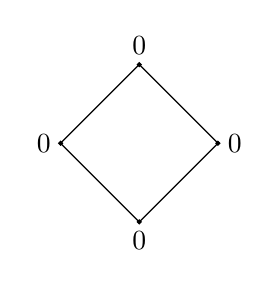
\begin{tikzpicture}
\draw (0,0) --(1,1);
\draw (1,1) --(2,0);
\draw (2,0) --(1,-1);
\draw (1,-1) --(0,0);
\draw[fill] (0,0) circle [radius=0.025];
\draw[fill] (1,1) circle [radius=0.025];
\draw[fill] (1,-1) circle [radius=0.025];
\draw[fill] (2,0) circle [radius=0.025];
\node [left] at (0,0) {0};
\node [above] at (1,1) {0};
\node [right] at (2,0) {0};
\node [below] at (1,-1) {0};
\end{tikzpicture}
\item[е)] Попробуйте описать группу циклических преобразований любого отрезка с нулевыми весами.
\end{description}
\item Считая, что мы определили допустимые преобразования цепей и циклов как графов, дайте определения допустимых преобразований произвольных графов.
\end{enumerate}

\bigskip



\task{Учимся считать}

$F$ - произвольное поле, $n\choose k$ --- число сочетаний из $n$ элементов по $k$.
\begin{enumerate}
\item  Посчитайте, чему равно
\begin{align*}
-{b + 1 \choose 0}{b + c \choose b - 1}{c + 1 \choose c - 1} & + {b + 1 \choose 1}{b + c \choose b}{c + 1 \choose c} -\\
 - & {b + 1 \choose 2}{b + c \choose b + 1}{c + 1 \choose c + 1}.
\end{align*}
Ответ будет заметно короче этого выражения!

\item Представьте следующие числа в виде произведения и частного некоторых факториалов: $${4 \choose 0}^3 - {4 \choose 1}^3 + {4 \choose 2}^3 - {4 \choose 3}^3 + {4 \choose 4}^3$$ и $${6 \choose 0}^3 - {6 \choose 1}^3 + {6 \choose 2}^3 - {6 \choose 3}^3 + {6 \choose 4}^3 - {6 \choose 5}^3 + {6 \choose 6}^3.$$

\item Попытайтесь как-то обобщить без строгого доказательства полученные результаты.

\item Посчитайте, чему равен коэффициент многочлена $[x^2y^2z^2](x-y)^2(y-z)^2(z-x)^2$, где $[\,]$ означает взятие коэффициента при соответствующем мономе. А $[x^2y^2z^2](x-y)(x-y-1)(y-z)(y-z-1)(z-x)(z-x-1)$? В каких целочисленных точках куба $(0 \leq x \leq 3) \times (0 \leq y \leq 3) \times (0 \leq z \leq 3)$ эти многочлены принимают ненулевые значения? Что можно сказать про значения этих многочленов в целых точках данного куба и про указанный коэффициент?

\item Докажите интерполяционную формулу Лагранжа: если $C$ - произвольное подмножество $F$ размера $d + 1$, а $f$ - многочлен степени не выше $d$, то $$f = \sum\limits_{a \in C}{f(a){\prod_{c \in C, c \neq a}\frac{x - c}{a - c}}}.$$

\item Пусть $f \in F[x_1,x_2]$ - многочлен от двух переменных суммарной степени $deg(f) \leq d_1 + d_2$, а $C_1,C_2$ - произвольные подмножества $F$ размера $|C_i| \geq d_i + 1$. Тогда $$\sum\limits_{c_1 \in C_1} \sum\limits_{c_2 \in C_2} \frac{f(c_1,c_2)}{\phi_1'(c_1)\phi_2'(c_2)} = [x_1^{d_1}x_2^{d_2}]f(x_1,x_2),$$ где $\phi_i(z) = \prod_{c\in C_i}{(z-c)}$.

\item Постарайтесь усилить и доказать теорему из пункта 6. Можете ли Вы придумать способ выразить коэффициент многочлена при произвольном мономе через его значение в заданных точках (как в предыдущем пункте, например)?

\item Постарайтесь посчитать, чему равен коэффициент многочлена $[x^ay^az^a](x-y)^a(y-z)^a(z-x)^a$ двумя разными способами и получить отсюда загадочное тождество.

\item Постарайтесь придумать тождество, обобщающее все тождества этой задачи, и доказать его. 



\end{enumerate}



\task{Разрезания куба}
\begin{enumerate}
\item Рассмотрим куб $3\times 3\times 3$. Мы хотим разрезать его на кубики $1\times 1\times 1$. За один раз можно сделать разрез в одной плоскости, при этом перед следующим разрезом можно переставлять в пространстве уже отрезанные части. За какое минимальное число разрезов можно справиться?
\item Рассмотрите теперь куб $n\times n\times n$. За сколько разрезаний можно справиться? Объясните, почему за меньшее число нельзя?
\item А сколькими разными способами можно произвести такое разрезание (способы различны, если на каком-то шаге от кубика отрезаны разные множества)? А если называть разрезания разными, когда на каком-то шаге в них отличаются наборы отрезанных фигур?
\item Рассмотрим равносторонний треугольник на плоскости с длиной стороны $n$. Мы хотим разрезать его на равносторонние треугольники с длинной стороны 1. За сколько разрезаний это возможно? Сколькими способами?
\item Рассмотрите аналогичную задачу для $d$-мерного куба и $d$-мерного симплекса.
\item Проверьте, что трёхмерный куб $n\times n \times n$ можно разрезать на $4n^3$ прямоугольных тетраэдров и $n^3$ правильных тетраэдров. Каково наименьшее число разрезаний?
\item Рассмотрите другие возможные разрезания. 
\end{enumerate}


\task{Маляры}

 Графом $G = (V,E)$ называется множество $V$ и симметричное отношение инцидентности $E\subset V\times V$. Множество $V$ называется множеством вершин, а $E$ --- множеством ребер. Если $E\cap \{(v,v)|v\in V\} = \varnothing$, то говорят, что в графе нет петель. Мы будем рассматривать только такие графы.

Правильной раскраской графа $G$ в $n$ цветов называется отображение $col: V\to [n] = \{1,2,\dots, n\}$ такое, что никаким двум инцидентным вершинам не сопоставляется один и тот же цвет, то есть $(v,v')\in E \Rightarrow col(v)\neq col(v')$. Хроматическим числом графа $G$ называется наименьшее $n$, для которого существует правильная раскраска в $n$ цветов. Хроматическое число обозначается $\chi(G)$.

Пусть $(M,d)$ --- метрическое пространство. Положим, $V = M$ и $E = \{(m,m')\in M\times M\ \mid\ d(m,m') = 1\}$. Тогда по определению $\chi(M) = \chi(G)$, где $G = (V,E)$.

Во всех последующих пунктах через $\mathbb R$ обозначается множество вещественных чисел, через $\mathbb R^n$ обозначается метрическое пространство, точки которого являются упорядоченными наборами из $n$ чисел, а расстояние определяется по формуле
$$
d((x_1,\dots,x_n), (y_1,\dots,y_n)) =\sqrt{ \sum\limits_{j = 1}^n(x_j-y_j)^2}.
$$
Все подмножества $\mathbb R^n$ считаются метрическими пространствами с индуцированной из $\mathbb R^n$ метрикой.

\begin{enumerate}

\item Докажите, что $\chi(\mathbb R^2)\geq 4$, то есть плоскость нельзя раскрасить в $3$ цвета. Предъявите раскраску плоскости в $7$ цветов: $\chi(\mathbb R^2)\leq 7$.

\item Докажите, что $\chi(\mathbb R^n)\geq n+2$.

\item Зафиксируем положительное число $\varepsilon < \sqrt{3/7}$. Покажите, что $5\leq \chi(\mathbb R^2\times [0,\varepsilon])\leq 7$.

\item Зафиксируем положительное число $\varepsilon < 10^{-3}$. Покажите, что $\chi(\mathbb R^2\times [0,\varepsilon]^2)\geq 6$

\item Зафиксируем простое число $p$. Через $\mathbb F_p$ будем обозначать поле из $p$ элементов. Пусть $n$ --- натуральное число, рассмотрим граф $G^p_n = (V^{(p)}_n,E^{(p)}_n)$, где $V^{(p)}_n = (\mathbb F_p)^n$, а $E^{(p)}_n = \{(v,w)\in V_n^{(p)}\times V^{(p)}_n\ \mid\ v\cdot w = 1\}$, где
$$
(v_1,\dots,v_n)\cdot(w_1,\dots,w_n) = \sum\limits_{j = 1}^nv_jw_j.
$$

 Оцените $\chi(G^2_n)$, $\chi(G^3_n)$ при больших $n$.


\item Оцените $\chi(G^p_n)$ при больших $n$ для произвольного $p$.

\end{enumerate}


\task{Как подгонять и не оплошать}

В некотором конкурсе участвуют $n$ команд из $k$ участников. Команды уже отыграли, и осталось лишь определить победителя. При равенстве очков одно место может распределиться среди нескольких команд (как на математической олимпиаде).

Каждый участник команды заработал некоторую оценку из интервала $[0,1]$. Таким образом, результаты команд, исходя из которых надо их упорядочить, записаны невозрастающими последовательностями из $k$ неотрицательных чисел. И для того, чтобы подвести итог, необходимо придумать функцию $f: \mathbb [0,1]^k\to \mathbb R$, которая будет вычислять окончательный результат каждой команды.

А теперь --- главный нюанс. Выбор этой функции целиком во власти жюри. Предположим, что некий член жюри, ответственный за выбор функции, пытается предложить капитанам команд подобрать $f$ таким образом, чтобы команда этого капитана не оказалась, ммм..., в последних рядах. 

Но не всё так просто. С одной стороны понятно, что стоит пообещать первое место наибольшему числу команд, однако, если ответственный обнадёжит тем, что потом не сможет сделать, то обиженная команда обязательно разболтает о его предложении.

Вдобавок, Комитетом По Защите Прав Олимпиадников установлены следующие правила: функция $f$ должна иметь вид
$$
f(x_1,\dots,x_k) =\left (\sum\limits_{j = 1}^kw_jx_j^l  \right )^{1/l}
$$
для некоторого вещественного числа $l\geq 1$ и весов $w_1\geq w_2\geq\dots\geq w_k> 0$.


\bigskip
\begin{enumerate}
\item Пусть $k = 3,\ n = 4$ и результаты оказались следующими:
$$\bar{l}
(0.3,0.1,0.1),\ (0.2,0.2,0.1),\ (0.15, 0.14, 0.14),\ (0.13,0.1,0.1).
\ear$$
Стоит ли обещать помощь последней команде?

\item
 Будем говорить, что $(x_1,\dots, x_k)$ мажорирует $(y_1,\dots,y_k)$, если $\sum\limits_{i = 1}^jx_i > \sum\limits_{i = 1}^jy_i$ для любого~$j$. Предположим, что ни для каких двух команд не верно, что результаты одной мажорируют результаты другой.

Какое максимальное число команд гарантировано можно вывести на первое место?

\item Пусть $A\subset [0,1]^k$ --- некоторое открытое подмножество. Вероятностью того, что результаты данной команды попали в множество $A$, будем считать $|A|$, где $|A|$ --- объем множества $A$. Результаты команд считаются независимыми в совокупности.

Пусть $k,n$ и некоторое натуральное число $j$ фиксированы. С какой вероятностью можно подобрать $l,w_1,\dots, w_k$ для того, чтобы вывести на первое место ровно $j$ команд?

\end{enumerate}





\task{Как бы поделить}
\begin{enumerate}
\item Многочлен $f(x)\in F[x]$ с коэффициентами из поля $F$ называется неприводимым, если все его делители в $F[x]$ имеют вид $c$, $cf(x)$, $c\in F\setminus\{0\}$. 
Покажите, что следующие многочлены неприводимы, как многочлены с рациональными коэффициентами:
\begin{description}
\item[а)] $x^2+2bx +1$ , где $b\in\mb{Z}$, $|b|>1$.
\item[б)] $x^4+1$.
\end{description}
\item Разложите на неприводимые множители $x^{18}-1$ над рациональными числами. Найдите нетривиальное разложение на множители числа $2^{18}-1$.
\item Хорошо известно, что многочлен $\Phi_n(x)=\prod_{(k,n)=1, k<n} (x-e^{2\text{π} i k/n})$ является многочленом с целыми коэффициентами и что $x^n-1=\prod_{d|n}\Phi_d(x)$. Покажите, что многочлен $\Phi_n(x)$ неприводим над $\mb{Q}$.
\item Для каких $n$ многочлен $\Phi_n$, взятый по модулю простого $p$ (что корректно, так как он с целыми коэффициентами), приводим в поле из $p$ элементов? Например, при $p=11$?
\item Покажите, что над полем из $p$ элементов многочлен $x^p-x+1$ неприводим. Покажите, что он является делителем $x^{p^p-1}-1$. Делителем какого $\Phi_d(x)$ является $x^p-x+1$?
\item Рассмотрим некоторый целочисленный многочлен $g(y)\in\mb Z[y]$. Например, $g(y)=ay^n$. Для каких $g(y)$ и $d$ многочлен $\Phi_d(g(y))$ не является неприводимым над $\mb{Q}$?
\item Что можно сказать, если вместо $\Phi_d(x)$ взять какой-то другой неприводимый многочлен? Можно ли взять $g(y)$ маленькой степени (меньше степени исходного многочлена)? Бесконечно ли число таких $g(y)$?
\end{enumerate}

\task{Выпуклые функции}
Напомним, что функция $F\colon\mb R^d\to\mb R$ называется выпуклой, если
$$\forall x,y\in\mb R^d,\,\, t\in [0,1]\,\,\,\, tF(x)+(1-t)F(y)\geq F(tx+(1-t)y).$$
\begin{enumerate}
\item Хорошо известно, что выпуклая функция из $\mb R$ в $\mb R$ непрерывна. Покажите, что это выполнено и в случае большей размерности.
\item Теперь рассмотрим ситуацию похитрее. Пусть $d=2$ и $f(x_1, x_2)$ выпукла по каждой координате в отдельности, то есть при фиксированном $x_1$ она выпукла, как функция от $x_2$ и наоборот. Покажите, что $f$ непрерывна.
\item Покажите то же самое для $d>2$.
\item Пусть $F$ выпукла и положительно однородна порядка 1, т.е. $F(\lambda x)=|\lambda|F(x)\,\,\forall x\in \mb R^d$. Покажите, что такая функция неотрицательна.

\item Пусть функция $F: \mathbb{R}^d \to \mb R$ является выпуклой по каждой переменной и положительно однородна порядка $1$. Докажите, что функция $F$ неотрицательна.

\item Функция $F$ называется липшицевой, если существует такая $L>0$, что $$|f(x)-f(y)|<L|x-y|\,\, \forall x,y\in \mb R^d.$$ Функция $F\colon \mb R^d\to \mb R$ называется субгармоничной, если для всякой точки $x_0$ и шарика $Q$ с центром в точке $x_0$ ${F(x_0)} \leq \frac{1}{\Vol(Q)} \int\limits_{Q} F(x) dx $, где $\Vol(Q)$ обозначает объём шара $Q$.

 Пусть функция $F: \mathbb{R}^{2d} \to \mb R$ липшицева, положительно однородна порядка $1$, и для каждого $j \in [1,d]$ субгармонична по переменным $(x_j, x_{j+d})$.  Докажите, что функция $F$ неотрицательна, если:
\begin{description}
\item[а)] $d$ равно единице.
\item[б)] $d$ --- произвольное натуральное число.

\end{description}

\item Постройте контрпример для случая нечётной размерности. Например, в $\mathbb{R}^3$.
\end{enumerate}